\begin{frame}{Test Classe Applicazione}
    
    \begin{figure}
        \centering
        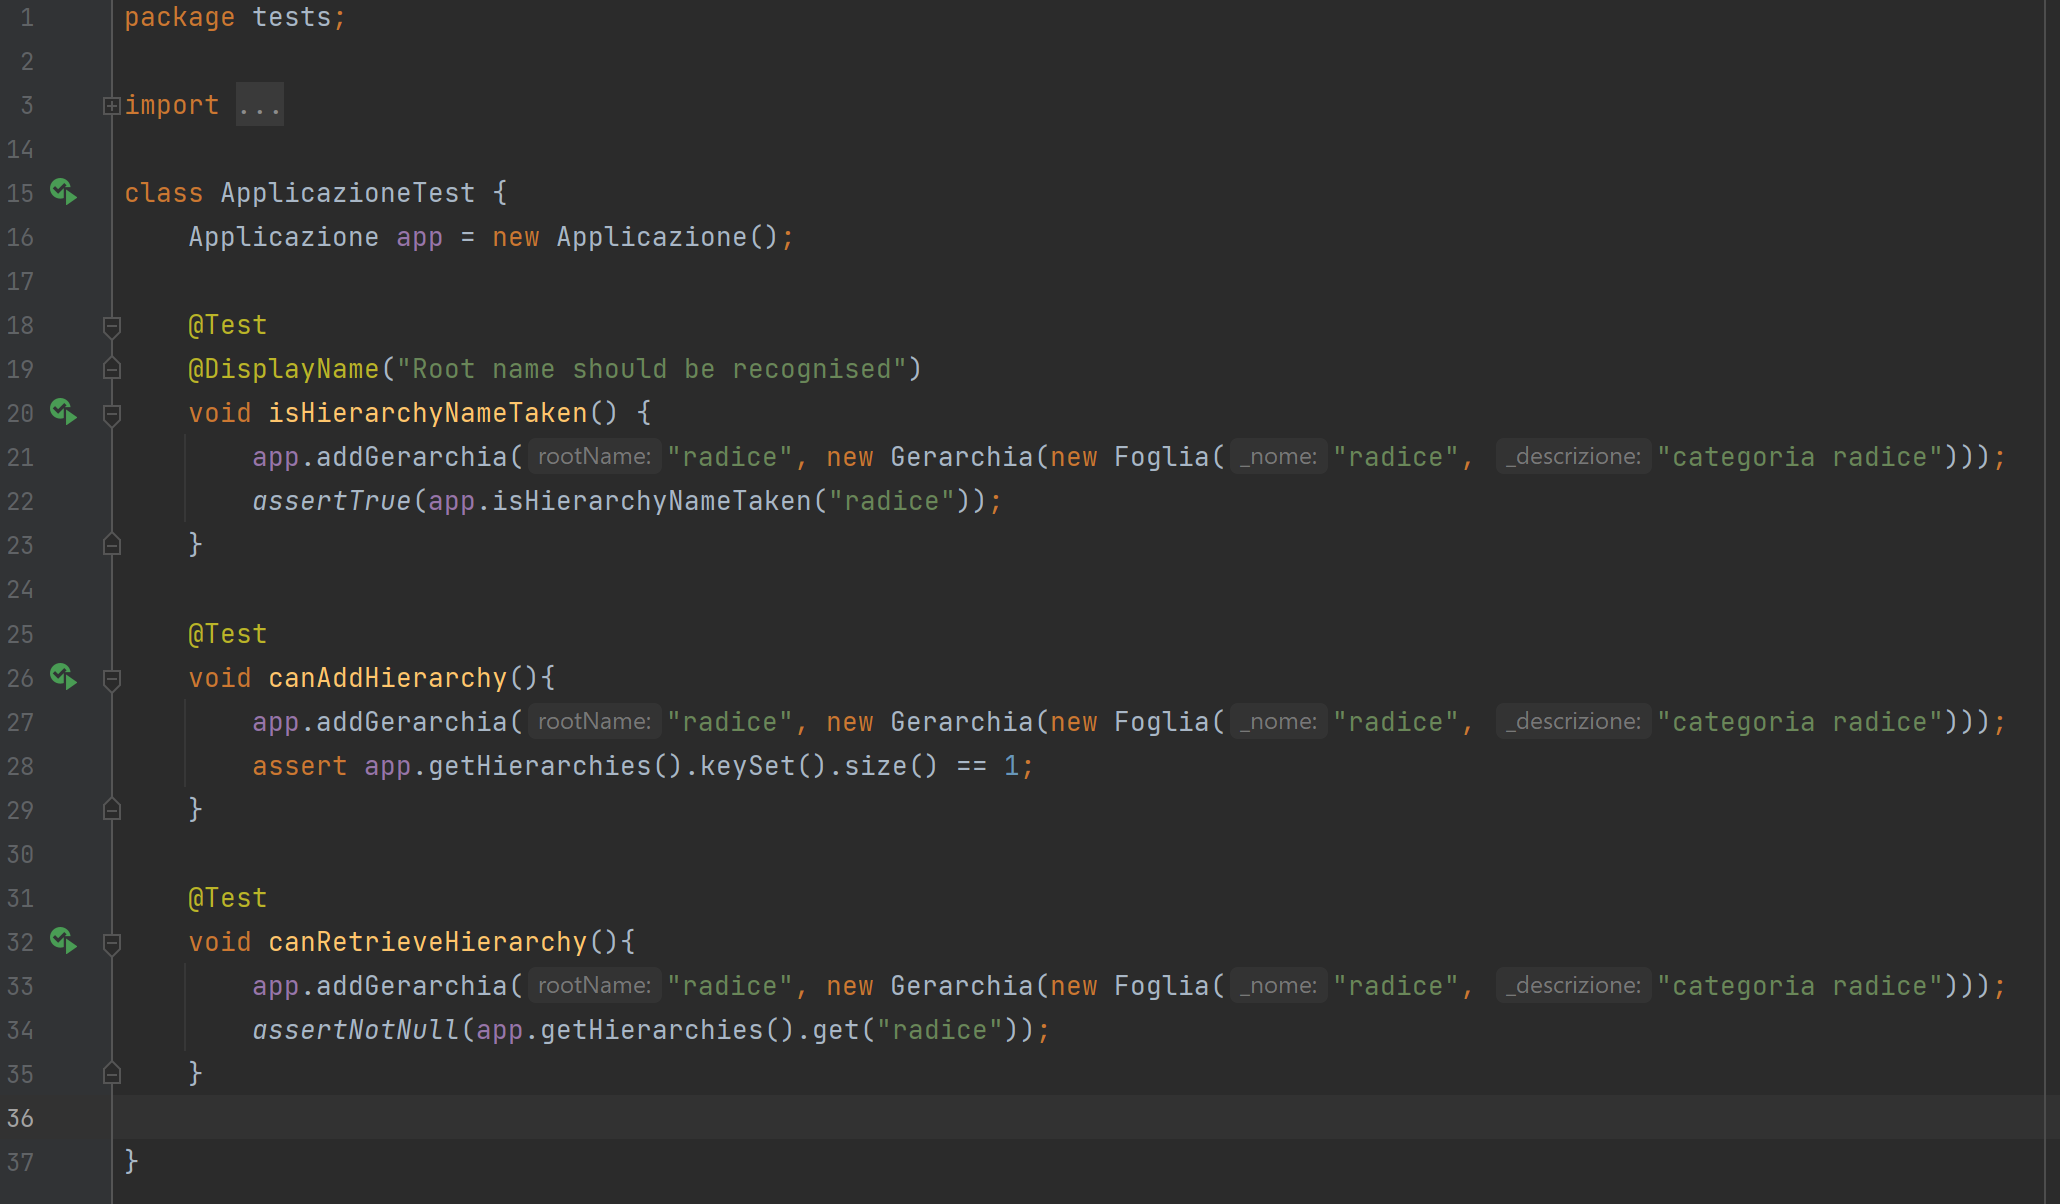
\includegraphics[width=.8\textwidth]{initial testing/testApplicazione.png}
    \end{figure}

    \note{
        I test eseguiti sulla classe Applicazione, così come sulle altre, sono stati effettuati selezionando i metodi principali dalla cui correttezza dipendeva in modo ingente la fattibilità del resto del codice.\bigskip

        \textbf{isHierarchyNameTaken()}

        Il test si assicura che, dopo aver inserito una gerarchia nell'applicazione, la verifica della presenza del nome della gerarchia inserita abbia esito positivo.\bigskip 

        \textbf{canAddHierarchy()}

        Il test si assicura che, dopo aver inserito una gerarchia nell'applicazione, la verifica della presenza di esattamente una gerarchia nell'applicazione abbia esito positivo.\bigskip

        \textbf{canRetrieveHierarchy()}

        Il test si assicura che, dopo aver inserito una gerarchia non \texttt{null} nell'applicazione, essa possa essere recuperata e che non venga restituito un valore \texttt{null}, come in effetti ci si aspetta.\\
    }    
\end{frame}

\begin{frame}{Test Classe CampoNativo}
    
\end{frame}

\begin{frame}{Test Classe Categoria}
    
\end{frame}

\begin{frame}{Test Classe ExchangeMessage}
    
\end{frame}

\begin{frame}{Test Classe IntervalloOrario}
    
\end{frame}

\begin{frame}{Test Classe Orario}
    
\end{frame}

\begin{frame}{Test Classe UserDataStore}
    
\end{frame}

\begin{frame}{Test Classe User}
    
\end{frame}